% Copyright (C) 2011 The ESPResSo project
%   Max-Planck-Institute for Polymer Research, Theory Group
%  
% This file is part of ESPResSo.
%   
% ESPResSo is free software: you can redistribute it and/or modify it
% under the terms of the GNU General Public License as published by the
% Free Software Foundation, either version 3 of the License, or (at your
% option) any later version.
%  
% ESPResSo is distributed in the hope that it will be useful, but
% WITHOUT ANY WARRANTY; without even the implied warranty of
% MERCHANTABILITY or FITNESS FOR A PARTICULAR PURPOSE.  See the GNU
% General Public License for more details.
%  
% You should have received a copy of the GNU General Public License
% along with this program.  If not, see <http://www.gnu.org/licenses/>.
%
\documentclass[
a4paper,                        % paper size
11pt,                           % font size
twoside,                        % two sided
footsepline,                    % add a line to separate the footer
headsepline,                    % add a line to separate the header
headexclude,                    % header does not belong to the text
footexclude,                    % footer does not belong to the text
pagesize,                       % set the pagesize in a DVI document
bibtotocnumbered,               % add the bibliography to the TOC
idxtotoc                        % add the index to the TOC
%openright,                      % start a new chapter on the right page
%,DIV12
%,draft
]{scrartcl}

\usepackage[draft]{varioref}    % defines \vref
\usepackage{hyperref}           % automatically creates links when
                                % using pdflatex, defines \url
\usepackage{ifpdf}              % defines \ifpdf
\usepackage{graphicx}           % handles graphics
\usepackage{makeidx}            % creates the index
\usepackage{color}              % use colors

\usepackage{amsmath}

\usepackage{calc}               % compute length
\usepackage{ifthen}             % provide ifthen
\usepackage{xspace}
\usepackage{units}
\usepackage[numbers]{natbib}

% For building the distribution docs, disable todo boxes.
%\usepackage[disable]{todonotes}
\usepackage{todonotes}

%%%%%%%%%%%%%%%%%%%%%%%%%%%%%%%%%%%%%%%%%%%%%%%%%%
%%%%%%%%%%%%%%%%%%%%%%%%%%%%%%%%%%%%%%%%%%%%%%%%%%
%%%%%%%%% New Commands and Environments %%%%%%%%%%
%%%%%%%%%%%%%%%%%%%%%%%%%%%%%%%%%%%%%%%%%%%%%%%%%%
%%%%%%%%%%%%%%%%%%%%%%%%%%%%%%%%%%%%%%%%%%%%%%%%%%
\newcommand{\es}{\mbox{\textsf{ESPResSo}}\xspace}
\newcommand{\ie}{\textit{i.e.}\xspace}
\newcommand{\eg}{\textit{e.g.}\xspace}
\newcommand{\etal}{\textit{et al.}\xspace}


%%%%%%%%%%%%%%%%%%%%%%%%%%%%%%%%%%%%%%%%%%%%%%%%%%
%%%%%%%%%%%%%%%%%%%%%%%%%%%%%%%%%%%%%%%%%%%%%%%%%%
%%%%%%%%%%%%%%%% Other Settings %%%%%%%%%%%%%%%%%%
%%%%%%%%%%%%%%%%%%%%%%%%%%%%%%%%%%%%%%%%%%%%%%%%%%
%%%%%%%%%%%%%%%%%%%%%%%%%%%%%%%%%%%%%%%%%%%%%%%%%%
\makeindex

%%%%%%%%%%%%%%%%%%%%%%%%%%%%%%%%%%%%%%%%%%%%%%%%%%
%%%%%%%%%%%%%%%%%%%%%%%%%%%%%%%%%%%%%%%%%%%%%%%%%%
%%%%%%%%%%%%%%%%% Main Document %%%%%%%%%%%%%%%%%%
%%%%%%%%%%%%%%%%%%%%%%%%%%%%%%%%%%%%%%%%%%%%%%%%%%
%%%%%%%%%%%%%%%%%%%%%%%%%%%%%%%%%%%%%%%%%%%%%%%%%%
\begin{document}
\titlehead{
  \begin{center}
    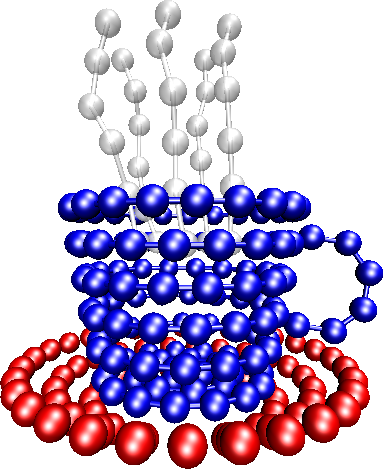
\includegraphics[width=5cm]{logo/transparentbg.png}
  \end{center}
}
%\subject{}
\title{\es Developer's Guide}
%\author{}
%\date{\today}
\maketitle

\tableofcontents
\listoftodos

\section{Development environment}
\label{sec:env}

\begin{itemize}
\item Autotools build system
\item \es homepage \url{http://espressomd.org}
\item Code hosting at GNU Savannah 
  \url{https://savannah.nongnu.org/projects/espressomd/}
\item Jenkins build server \url{http://espressomd.org/jenkins}
\end{itemize}

\section{Getting into contact}

The first thing that you should do when you want to start to
participate is to get into contact with the \es developers. To do
that, subscribe to the developers' mailing list at
\url{http://lists.nongnu.org/mailman/listinfo/espressomd-devel} and
write a short email to the list address
\texttt{espressomd-devel@nongnu.org} where you state your experience
with simulations and programming and the things that you would like to
do in \es. We do not bite, and we are happy about anybody who wants to
participate!

\section{Required development tools}
\label{sec:requirements}

If you want to participate in the development of \es, you will require
the following tools depending on what tasks you want to perform:

\begin{itemize}
\item To be able to access the development version of \es, you will
  need the distributed versioning control system
  Git\footnote{\url{http://git-scm.com/}}.  Section \vref{sec:git}
  contains documentation on how we employ git.
\item To build \es from the development sources, you will need not too
  old versions of the ``GNU autotools'' (\ie
  automake\footnote{\url{http://www.gnu.org/software/automake/}} and
  autoconf\footnote{\url{http://www.gnu.org/software/autoconf/autoconf.html}})
  installed on your system. Section \vref{sec:build_devel} contains
  information on how to build the development code, section
  \vref{sec:build_system} contains details on how the build system
  works.
\item To be able to compile the User's Guide or the Developer's Guide,
  you will need a \LaTeX-installation (all recent ones will do). For
  details, refer to chapter \vref{sec:docs}.
\item To compile the Doxygen code documentation, you will need to have
  the tool \textsc{Doxygen}\footnote{\url{http://www.doxygen.org/}}.
\end{itemize}

All of these tools should be easy to install on most Unix operating
systems.

\section{Using git}
\label{sec:git}

\section{Building the development code}
\label{sec:build_devel}

\begin{itemize}
\item Use \texttt{bootstrap.sh} before building the code.
\item Use configure with \texttt{--enable-maintainer-mode}.
\item Possible targets of \texttt{make}
  \begin{itemize}
  \item \texttt{check}
  \item \texttt{dist}
  \item \texttt{doc}
  \item \texttt{ug}
  \item \texttt{dg}
  \item \texttt{doxygen}
  \item \texttt{tutorials}
  \item \texttt{distcheck}
  \item \texttt{clean}, \texttt{distclean}
  \end{itemize}
\end{itemize}

\section{The build system}
\label{sec:build_system}

The build system of ESPResSo makes use of the GNU autotools suite
consisting of
automake\footnote{\url{http://www.gnu.org/software/automake/}} and
autoconf\footnote{\url{http://www.gnu.org/software/autoconf/autoconf.html}}.
If you want to use the development source code of ESPResSo, you first
need to install both of these tools.

The central source files of the build system are the following:
\begin{itemize}
\item \texttt{configure.ac}
\item \texttt{config/*.m4}
\item \texttt{Makefile.am}
\item the different \texttt{Makefile.am} in the subdirectories
\end{itemize}

To change the behaviour of the build system, you have to modify any
these files.

\subsection{Running \texttt{bootstrap.sh}}

The script \texttt{bootstrap.sh} in the top level source directory can
be used to run \texttt{automake}, \texttt{autoconf} and the associated
tools to generate the \texttt{configure} script and the
\texttt{Makefile.in} used during compilation.  Once
\texttt{bootstrap.sh}, the \es development code can be build and used
like the release code.

\subsection{Creating a distribution package}

As described in the User's Guide, to create a \texttt{.tar.gz}
distribution file that contains all required files, you can simply run
\texttt{make dist}. This will bundle all files and put them into an
archive with the name
\texttt{espresso-\textit{version}\texttt{.tar.gz}}.

Even better, you can also run \texttt{make distcheck}. This will not
only create the distribution file, but it will also thoroughly check
the created distribution, \ie it will try to 
\begin{itemize}
\item unpack the distro into a new directory
\item configure and build it (\texttt{configure})
\item run the testsuite (\texttt{make check})
\item install it into a new directory (\texttt{make install})
\item uninstall it (\texttt{make uninstall})
\end{itemize}
Whenever something goes wrong in these checks, it will give an error
message that describes the problem. When everything goes fine, you can
be relatively sure that you have a useful \es distribution
package.

In some cases, it might be necessary to pass some options to the run
of \texttt{configure} done by \texttt{make distcheck}>. To do that,
you can set the environment variable
\texttt{DISTCHECK\_CONFIGURE\_FLAGS} to the required options.

\paragraph{Example}
\begin{verbatim}
DISTCHECK_CONFIGURE_FLAGS="--without-mpi CPPFLAGS=\"-I /usr/include/tcl8.4\"" \
  make distcheck
\end{verbatim}

\section{The testsuite}
\label{sec:testsuite}

\begin{itemize}
\item How to write tests?
\item How they are called (\texttt{runtest.sh})
\end{itemize}



\printindex

\end{document}
